\documentclass{article}
\usepackage[utf8]{inputenc}
\usepackage{amsmath}
\usepackage{listings}
\usepackage{color}
\usepackage{graphicx}
\usepackage[margin=1in]{geometry}
\usepackage{hyperref}
\usepackage{gensymb}
\graphicspath{ {} }

\definecolor{dkgreen}{rgb}{0,0.6,0}
\definecolor{gray}{rgb}{0.5,0.5,0.5}
\definecolor{mauve}{rgb}{0.58,0,0.82}

%\lstset{frame=tb,
%  language=c,
%  aboveskip=3mm,
%  belowskip=3mm,
%  showstringspaces=false,
%  columns=flexible,
%  basicstyle={\small\ttfamily},
%  numbers=left,
%  numberstyle=\tiny\color{gray},
%  keywordstyle=\color{blue},
%  commentstyle=\color{dkgreen},
%  stringstyle=\color{mauve},
%  breaklines=true,  
%  breakatwhitespace=true,
%  tabsize=2
%}



\lstset{
  language=C,                % choose the language of the code
  numbers=left,                   % where to put the line-numbers
  stepnumber=1,                   % the step between two line-numbers.        
  numbersep=20pt,                  % how far the line-numbers are from the code
  backgroundcolor=\color{white},  % choose the background color. You must add \usepackage{color}
  showspaces=false,               % show spaces adding particular underscores
  showstringspaces=false,         % underline spaces within strings
  showtabs=false,                 % show tabs within strings adding particular underscores
  tabsize=4,                      % sets default tabsize to 2 spaces
  captionpos=b,                   % sets the caption-position to bottom
  breaklines=true,                % sets automatic line breaking
  breakatwhitespace=true,         % sets if automatic breaks should only happen at whitespace
  title=\lstname,                 % show the filename of files included with \lstinputlisting;
    aboveskip=1mm,
  belowskip=1mm,
   basicstyle={\ttfamily},
}


\title{\textbf{Line Tracking Robot}\\ ECE 3411 \\ Final Project}
\author{Brian Marquis\\ David Paquette \\ \\ \today}
\date{}

\begin{document}

\maketitle

\tableofcontents
 \newpage
\section{Objective}
The goal of this project is to implement a line follower using the Redbot hardware and the AVR ISA. 
\section{Control Design}
The block diagram below shows an overview of our control strategy.
\subsection{Control Overview}
\begin{center}
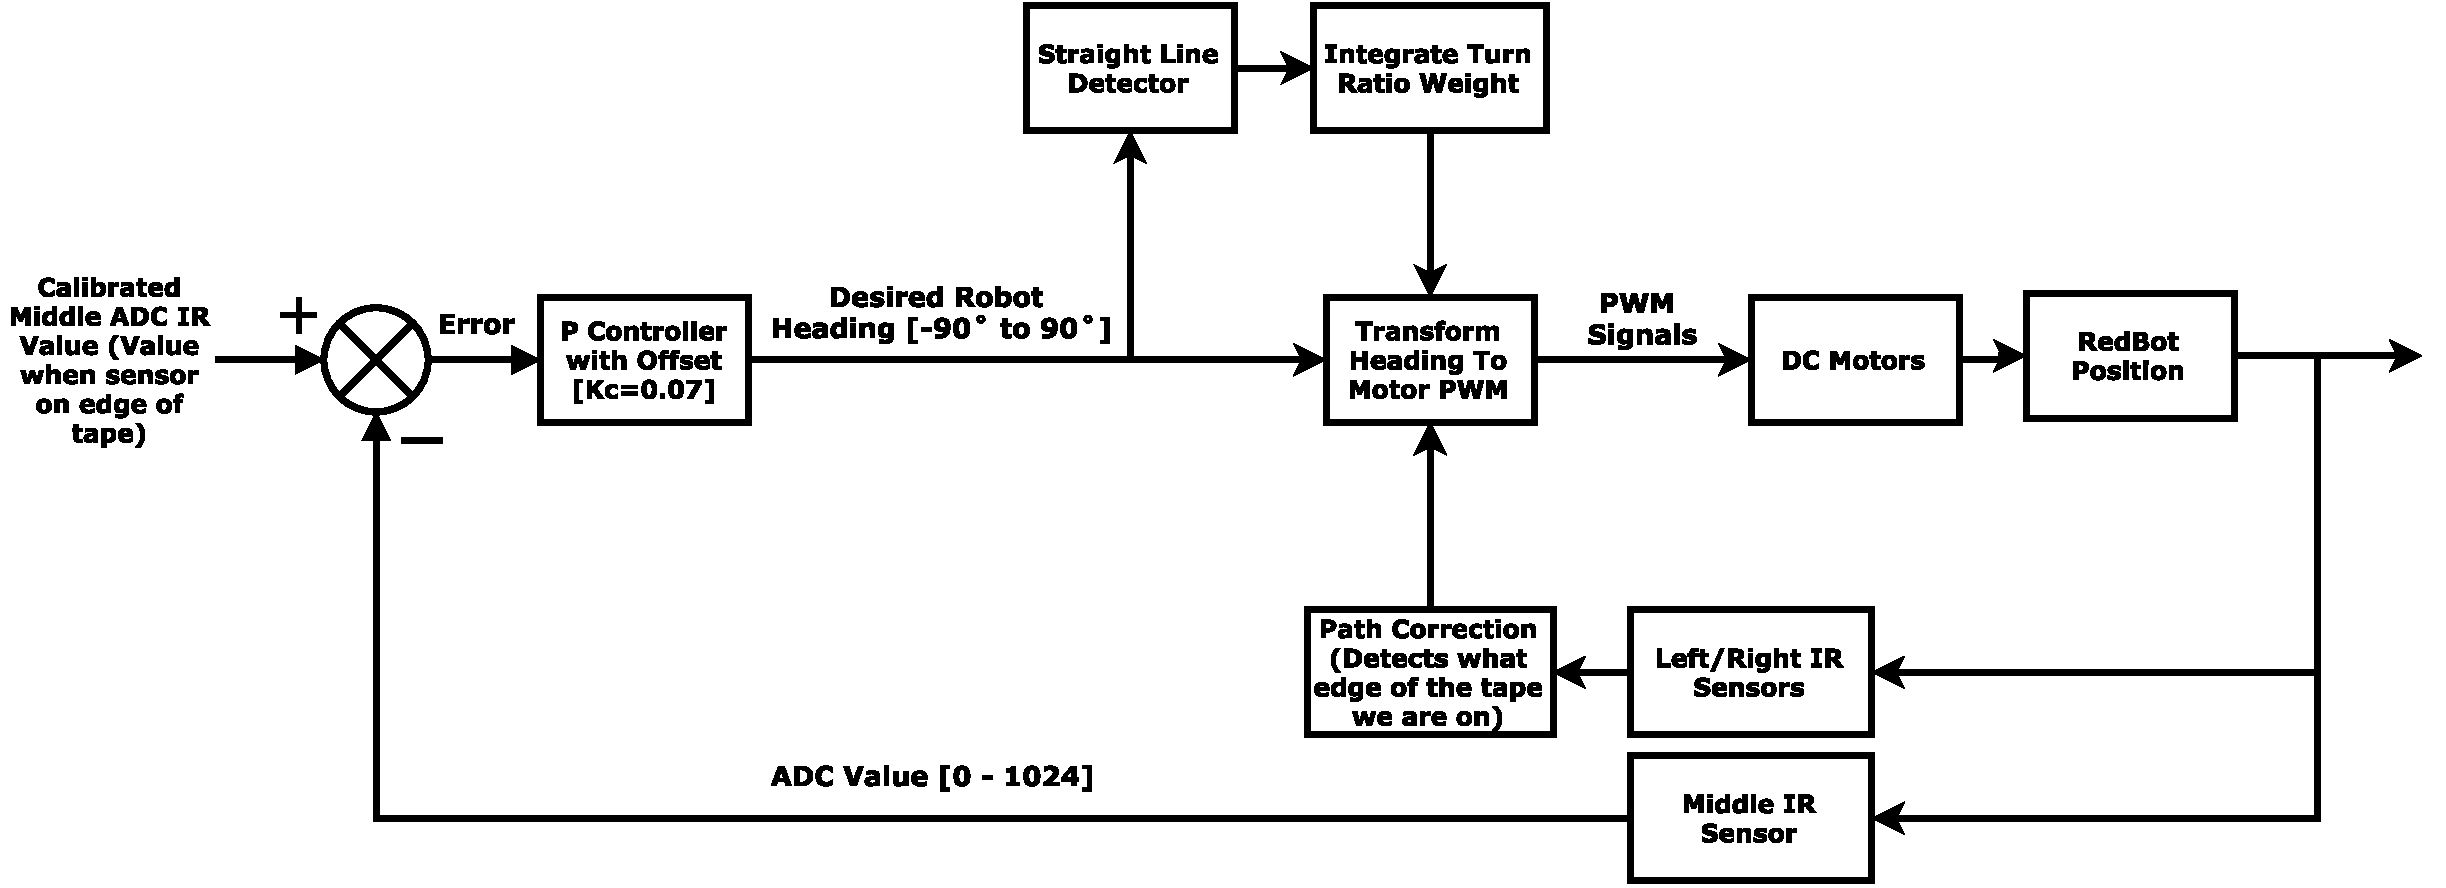
\includegraphics[scale=.43]{BD}
\centering
\end{center}
\textbf{FIG1.} Block diagram of controller overview. 

\subsection{PID Controller Implementation}

Instead of using a threshold based on/off controller for maintaining our position on the line we used a PID controller. We are using the discrete non-interactive PID control algorithm described by
\[ y[n+1] = K_C\left(e[n]+\frac{T_s}{T_I}\sum_{n} e[n]+T_D\frac{e[n]-e[n-1]}{T_s} \right)\]
Where
  \[e[n]=r[n]-m[n]\]
   and where $K_c$ is the controller gain, $T_I$ is the integral time,  $T_D$ is the derivative time,  $T_s$ is the sampling rate, $y[n]$ is the controller output, $r[n]$ is our set point or reference signal and $m[n]$ is our middle sensor measurement. The implementation can be seen below in code sample 1. To prevent the integral term from continually summing to positive or negative infinity (which in practice would cause the summing variable to overflow back to zero) we included an anti-windup feature in the controller implementation. To prevent unrealistic controller values we saturate the controller output at plus/minus 90\degree. The -90\degree  corresponds to a "complete left turn", meaning the left wheel turns off and the right wheel is set to full speed. Plus 90\degree  causes a complete right turn. 0\degree  represents both wheels turning at the same speed, causing the robot to drive in a straight line at the controller's set offset value.\\\\

\begin{lstlisting}
void PIDControllerComputeOutput(PIDController *controller, float processVariable) {
	//compute error
	controller->error = controller->processVariableSetPoint - processVariable;
	//compute integral component
	if(controller->integralTime) { //prevent divide by zero error
    	controller->errorIntegral = (1 / controller->integralTime) * controller->samplingPeriod * controller->error + controller->errorIntegral;
    	//wind up protection
    	controller->errorIntegral = controller->errorIntegral < controller->minControllerOutput*100 ? controller->minControllerOutput*100 : controller->errorIntegral;
    	controller->errorIntegral = controller->errorIntegral > controller->maxControllerOutput*100 ? controller->maxControllerOutput*100 : controller->errorIntegral;
	}
	//compute derivative term
	float derivativeComponent = (controller->derivativeTime*(controller->previousError - controller->error))/controller->samplingPeriod;
	//compute controller output Kc*(e+Ts/Ti*int(e)+Td*d(e)/Ts)
	controller->controllerOutput = controller->controllerGain * (controller->error + controller->errorIntegral + derivativeComponent);
	controller->previousError = controller->error;
	controller->controllerOutput = controller->controllerOutput < controller->minControllerOutput ? controller->minControllerOutput : controller->controllerOutput;
	controller->controllerOutput = controller->controllerOutput > controller->maxControllerOutput ? controller->maxControllerOutput : controller->controllerOutput;
}
\end{lstlisting}
\textbf{Code sample 1.} (PIDController.c) PID controller compute output implementation with anti-windup and controller output saturation.

\subsection{Path Correction}
The Redbot is designed to keep its middle IR sensor halfway on the tape.  If the left or right sensors detect black, indicating that the center has veered off of its mark, the Redbot will align its center sensor to the closest side of the tape.  This helps the Redbot to find the path again if it veers off of the path. \\
\begin{lstlisting}
 if(direction > 0 && LeftSensor > 700) direction *= -1;
 if(direction < 0 && RightSensor > 700) direction *= -1;
\end{lstlisting}
\textbf{Code sample 2.} (main.c) Path correction implementation.
\\\\
If the left or right IR sensor detects black, the direction parameter (1 or -1) will multiply itself by negative one to invert its current direction.  When the direction is inverted, the Redbot will now seek to align its middle sensor with the other side of the tape.

\subsection{Straight Line Detection and Acceleration}
The Redbot is designed to keep its middle IR sensor halfway on the tape.  If the left or right sensors detect black, indicating that the center has veered off of its mark, the Redbot will align its center sensor to the closest side of the tape.  This helps the Redbot to find the path again if it veers off of the path.
\\\\
\begin{lstlisting}
void setLeftMotorDutyCycle(float dutyCycle){
    Left_duty_cycle = (int)((float)(Left_time_period)*(dutyCycle/100.0));
}

void setRightMotorDutyCycle(float dutyCycle){
    Right_duty_cycle = (int)((304.0)*(dutyCycle/100.0));
}

void setSpeeds(float error)
{
    if(abs(error) < 11.2){
   	 if(turnRatio>0){
   		 turnRatio-=0.05;
   	 }
    } else if(abs(error) < 20){
   	 if(turnRatio<TURN_POWER) {
   		 turnRatio+=0.10;
   	 }
    } else {
   	 turnRatio = TURN_POWER;
    }
    setLeftMotorDutyCycle(((direction)*-1*error/90.0)*turnRatio+(100.0-turnRatio));
    setRightMotorDutyCycle(direction*(error/90)*turnRatio+(100.0-turnRatio));
}
\end{lstlisting}
\textbf{Code sample 3.} (main.c) Controller heading output to PWM and straight line acceleration implementation. (The parrameter $error$ is not the controller error, but the controller output, it was poorly named)
\\\\
The setLeftMotorDutyCycle and setRightMotorDutyCycle set the duty cycle for each motor.  The setSpeeds method first checks the previous error value and if it is less than the lower threshold, 11.2, the turn ratio will decrease linearly by 0.05.  Decreasing the turn ratio will increase the linear speed and decrease the turn speed.  This is used to speed up the Redbot when the path appears to be a straightaway.  Otherwise, if the error is greater than 11.2 but less than 20, the turn ratio will increase linearly to provide more power to turn the Redbot.  This function is used to gradually slow down the Redbot when it begins to detect a curve.  Finally, if the error is greater than 20, the redbot will reset its turn ratio to an optimal value for curved paths.  Next, setLeftMotorDutyCycle and setRightMotorDutyCycle are called using the error and the calculated turn ratio.

\subsection{Controller Tuning}
We tuned the controller using trial and error. The Redbot performed adequately with a Kc of 0.07. Because the integral and derivative terms introduce more complexity into the trial and error tuning process, we decided to only use a proportional controller. We also tuned the straight line acceleration and turn ratio weights by trial and error. 


\section{Sensor Overview}
\subsection{ADC Initialization}
The ADC is initially set to read from channel 6 with a prescaler of 2 so that the conversion is as fast as possible.  In addition, the ADC interrupt is enabled so that the active channel can be changed to read other sensors.
\begin{lstlisting}
void initADC(){
    //init the A to D converter
    ADMUX |= (1<<MUX1)|(1<<MUX2) |(1<< REFS0);
    ADCSRA = (1<<ADEN) | (1<<ADPS1)|(1<<ADIE);
}
\end{lstlisting}
\textbf{Code sample 4.} (main.c) ADC inits.

\subsection{ADC Channel Switching}
A simple state machine is used inside the ADC ISR to change the current sensor to be read.  The middle sensor is read first.  Next, the left sensor then the right sensor are read.

\begin{lstlisting}
ISR( ADC_vect ) {
    switch(adcChannel){
   	 case MIDDLE_SENSOR:
   		 ADMUX = 0;
   		 ADMUX |= IR_l;
   		 adcChannel = LEFT_SENSOR;
   		 break;
   	 case LEFT_SENSOR:
   		 ADMUX = 0;
   		 ADMUX|= IR_r;
   		 adcChannel = RIGHT_SENSOR;
   		 break;
   	 case RIGHT_SENSOR:
   		 ADMUX = 0;
   		 ADMUX|= IR_m;
   		 adcChannel = MIDDLE_SENSOR;
   		 break;
    }
}
\end{lstlisting}
\textbf{Code sample 5.} (main.c) ADC channel switching.
\subsection{Reading from the ADC}
To read each sensor, the ADC high and low registers are read when the conversion completes.  Then the ISR is invoked which changes the current ADC channel and then next read occurs.  This process takes place three times in this method to read the middle, left, and right IR sensors with one call.
\begin{lstlisting}
float readAnalogVoltage(){

    ADCSRA |= (1 << ADSC);
    while((ADCSRA & (1<<ADSC)));
    int adcIn = (ADCL);
    adcIn |= ( ADCH << 8 );

    ADCSRA |= (1 << ADSC);
    while((ADCSRA & (1<<ADSC)));
    RightSensor = (ADCL);
    RightSensor |= ( ADCH << 8 );


    ADCSRA |= (1 << ADSC);
    while((ADCSRA & (1<<ADSC)));
    LeftSensor = (ADCL);
    LeftSensor |= ( ADCH << 8 );

    return adcIn;
}

\end{lstlisting}
\textbf{Code sample 6.} (main.c) Reading the ADC.
\section{PWM and Motor Control}
\subsection{PWM Initialization}
Timer 0 is configured to produce a 50kHz PWM signal to OC0B.  The duty ratio can be controlled by adjusting the OCR0B register.  In addition, Timer 1 is also configured to produce a 50kHz PWM signal.  The frequency of timer 1 is controlled by the OCR0A and prescaler values.  Finally, the PWM output is handled in the output compare interrupt service routines by toggling the desired pin to drive the motors.
\begin{lstlisting}
//Set up Timer 0 for PWM at about 50kHz
   	 TCCR0A |= (1<<WGM01)|(1<<WGM00)|(1<<COM0B1);//Fast PWM Mode
   	 OCR0B = Left_duty_cycle; //Duty ratio currently at max value 0-255
   	 TIMSK0 |= (1<<OCIE0B);
   	 TCCR0B |= (1<<CS00);//prescaler of 1

   	 //Set up Timer 1 for Right Motor PWM
   	 TCCR1A |= (1<<WGM10)|(1<<WGM11);   	 //Fast PWM
   	 TCCR1B |= ((1<<WGM12)|(1<<WGM13)|(1<<CS10));   	 // Prescaler = 1
   	 TIMSK1 |= ((1<<OCIE1B)|(1<<OCIE1A));
   	 OCR1A = Right_time_period;
   	 OCR1B = Right_duty_cycle;

\end{lstlisting}
\textbf{Code sample 7.} (main.c) PWM inits.
\subsection{PWM Modulation}
\begin{lstlisting}
ISR(TIMER0_COMPB_vect)
{
    OCR0B = Left_duty_cycle;
}
ISR (TIMER1_COMPA_vect)
{
    OCR1B = Right_duty_cycle;
    Motor_Bank |= (1<<Right_PWM);
}

ISR (TIMER1_COMPB_vect)
{
    Motor_Bank &= ~(1<<Right_PWM);
}
\end{lstlisting}
\textbf{Code sample 8.} (main.c) PWM modulation. \\\\
These ISRs are used to update the duty ratio for each PWM signal and toggle the desired pin to drive the motors. \\\\
\subsection{Motor Control}
\begin{lstlisting}
void stopMotors()
{
    Motor_Bank &= ~((1<<Left_Mode_1)|(1<<Left_Mode_2)|(1<<Right_Mode_1));    //put both motors in stop mode
    Motor_Bank2 &= ~(1<<Right_Mode_2);
    Left_duty_cycle = 0;
    Right_duty_cycle = 0;
}

void motorForward()
{
    Motor_Bank |= (1<<Left_Mode_2)|(1<<Right_Mode_1);    //put both motors in forward mode
    Motor_Bank &= ~(1<<Left_Mode_1);    //put both motors in forward mode
    Motor_Bank2 &= ~(1<<Right_Mode_2);
}

void rightForward()
{
    Motor_Bank |= (1<<Right_Mode_1);
    Motor_Bank2 &= ~(1<<Right_Mode_2);
}

void leftForward()
{
    Motor_Bank |= (1<<Left_Mode_1);
    Motor_Bank &= ~(1<<Left_Mode_2);
}

void initMotors()
{
    motorForward();
    Left_duty_cycle = 0;//Left_time_period/5;
    Right_duty_cycle = 0;//Right_time_period/5;   	 //MAX SPEED
}

void leftBrake()
{
    Motor_Bank|=(1<<Left_Mode_1)|(1<<Left_Mode_2);
    Left_duty_cycle = 0;
}

void rightBrake()
{
    Motor_Bank|=(1<<Right_Mode_1)|(1<<Right_Mode_2);
    Right_duty_cycle = 0;
}

void leftReverse()
{
    Motor_Bank &= ~((1<<Left_Mode_1));
    Motor_Bank |= (1<<Left_Mode_2);   	 //put left motor in reverse mode
    //keep left PWM the same
}

void rightReverse()
{
    Motor_Bank &= ~((1<<Right_Mode_1));
    Motor_Bank2 |= (1<<Right_Mode_2);   	 //put right motor in reverse mode
    //keep right PWM the same
}

void Reverse()
{
    //put both motors in reverse mode but keep speed the same for now
    Motor_Bank &= ~((1<<Left_Mode_1)|(1<<Right_Mode_1));
    Motor_Bank |= (1<<Left_Mode_2)|(1<<Right_Mode_2);
}

\end{lstlisting}
\textbf{Code sample 9.} (main.c) Motor direction control.
\\\\
While most of these methods are not used in this source code, they simplify the process of changing the motor modes.  These methods simply set the control pins for each motor properly to put each motor in the desired state.
\\\\
\section{Conclusions}
While our design did follow the lines as intended, it could have handled some of the sharper turns better and the straightaway algorithm could have been optimized.  If we had more time, we would have tried to perhaps reverse one wheel when turning to allow for better handling.  In addition, we would have tried to use the encoders for the straightaway with a simple controller to keep the angular velocities equal.  This would allow the Redbot to travel straight as fast as possible in a straight line.
\\\\
\section{Complete Source Code}
\subsection{main.c}
\begin{lstlisting}
#include <avr/interrupt.h>
#define F_CPU 16000000UL /* Tells the Clock Freq to the Compiler. */
#include <avr/io.h> /* Defines pins, ports etc. */
#include <stdio.h>
#include "PIDController.h"
#include <stdlib.h>
PIDController motorRatioController;

volatile int controllerTimer = 0.0;
volatile float motorControllerSetpoint = 450.0;
volatile float CONTROLLER_GAIN = 0.07; // 0.07 for good line tracking at 0.55 turn ratio power
volatile float CONTROLLER_INTEGRAL_TIME = 0;//0.15; //seconds
volatile float CONTROLLER_DERIVATIVE_TIME = 0; //seconds
volatile float CONTROLLER_MIN_OUTPUT = -90.0;
volatile float CONTROLLER_MAX_OUTPUT = 90.0;
volatile float CONTROLLER_SAMPLING_PERIOD = 0.001;
volatile float INITIAL_CONTROLLER_OFFSET = 0.0;
volatile float direction = -1;
#define Left_PWM 5
#define Right_PWM 6

#define MIDDLE_SENSOR 0
#define LEFT_SENSOR 1
#define RIGHT_SENSOR 2


#define Left_Mode_1 2
#define Right_Mode_1 7

#define Left_Mode_2 4
#define Right_Mode_2 0

#define Motor_DDR DDRD
#define Motor_Bank PORTD
#define Motor_DDR2 DDRB
#define Motor_Bank2 PORTB
// straight values : L = 150 R = 159
volatile uint16_t Left_time_period = 255;
volatile uint16_t Left_duty_cycle = 80; // 255 max

volatile uint16_t Right_time_period = 319;
volatile uint16_t Right_duty_cycle = 120;    //0-317 (Highest Duty Ratio)

#define TURN_POWER 55.0 //40 for line, 55 for arbitrary path

volatile float turnRatio = TURN_POWER;

void InitTimer1();
void initADC();
void setSpeeds(float error);

#define IR_m (1<<MUX1)|(1<<MUX2)|(1<<REFS0)
#define IR_l (1<<MUX1)|(1<<REFS0)
#define IR_r (1<<MUX0)|(1<<MUX1)|(1<<REFS0)

volatile uint16_t LeftSensor;
volatile uint16_t RightSensor;

volatile int adcChannel = 0;

void inits(void)
{
   	 //Set up Data Direction Registers
   	 Motor_DDR |= (1<<Left_PWM)|(1<<Right_PWM)|(1<<Left_Mode_1)|(1<<Right_Mode_1)|(1<<Left_Mode_2);
   	 Motor_DDR2 |=(1<<Right_Mode_2);

   	 //Set up Timer 0 for PWM at about 50kHz
   	 TCCR0A |= (1<<WGM01)|(1<<WGM00)|(1<<COM0B1);//Fast PWM Mode
   	 OCR0B = Left_duty_cycle; //Duty ratio currently at max value 0-255
   	 TIMSK0 |= (1<<OCIE0B);
   	 TCCR0B |= (1<<CS00);//prescalar of 1

   	 //Set up Timer 1 for Right Motor PWM
   	 TCCR1A |= (1<<WGM10)|(1<<WGM11);   	 //Fast PWM
   	 TCCR1B |= ((1<<WGM12)|(1<<WGM13)|(1<<CS10));   	 // Prescalar = 1
   	 TIMSK1 |= ((1<<OCIE1B)|(1<<OCIE1A));
   	 OCR1A = Right_time_period;
   	 OCR1B = Right_duty_cycle;


   	 //Set up Timer 2 as a 1ms clock
   	 TCCR2A |= (1<<WGM21);    //CTC Mode
   	 OCR2A = 249;
   	 TIMSK2 |= (1<<OCIE2A);
   	 TCCR2B |= (1<<CS22);  //64 prescalar */
   	 initADC();
   	 motorRatioController = PIDControllerCreate(motorControllerSetpoint,
   	 CONTROLLER_GAIN, CONTROLLER_INTEGRAL_TIME, CONTROLLER_DERIVATIVE_TIME,
   	 CONTROLLER_MIN_OUTPUT,CONTROLLER_MAX_OUTPUT, CONTROLLER_SAMPLING_PERIOD,
   	 INITIAL_CONTROLLER_OFFSET);
   	 sei();
}

ISR( ADC_vect ) {
    switch(adcChannel){
   	 case MIDDLE_SENSOR:
   		 ADMUX = 0;
   		 ADMUX |= IR_l;
   		 adcChannel = LEFT_SENSOR;
   		 break;
   	 case LEFT_SENSOR:
   		 ADMUX = 0;
   		 ADMUX|= IR_r;
   		 adcChannel = RIGHT_SENSOR;
   		 break;
   	 case RIGHT_SENSOR:
   		 ADMUX = 0;
   		 ADMUX|= IR_m;
   		 adcChannel = MIDDLE_SENSOR;
   		 break;
    }
}

float readAnalogVoltage(){

    ADCSRA |= (1 << ADSC);
    while((ADCSRA & (1<<ADSC)));
    int adcIn = (ADCL);
    adcIn |= ( ADCH << 8 );

    ADCSRA |= (1 << ADSC);
    while((ADCSRA & (1<<ADSC)));
    RightSensor = (ADCL);
    RightSensor |= ( ADCH << 8 );


    ADCSRA |= (1 << ADSC);
    while((ADCSRA & (1<<ADSC)));
    LeftSensor = (ADCL);
    LeftSensor |= ( ADCH << 8 );

    return adcIn;
}

ISR(TIMER2_COMPA_vect) {
    controllerTimer++;
}

void initADC(){
    //init the A to D converter
    ADMUX |= (1<<MUX1)|(1<<MUX2) |(1<< REFS0);
    ADCSRA = (1<<ADEN) | (1<<ADPS1)|(1<<ADIE);
}

ISR(TIMER0_COMPB_vect)
{
    OCR0B = Left_duty_cycle;
}
ISR (TIMER1_COMPA_vect)
{
    OCR1B = Right_duty_cycle;
    Motor_Bank |= (1<<Right_PWM);
}

ISR (TIMER1_COMPB_vect)
{
    Motor_Bank &= ~(1<<Right_PWM);
}

void setLeftMotorDutyCycle(float dutyCycle){
    Left_duty_cycle = (int)((float)(Left_time_period)*(dutyCycle/100.0));
}

void setRightMotorDutyCycle(float dutyCycle){
    Right_duty_cycle = (int)((304.0)*(dutyCycle/100.0));
}

void setSpeeds(float error)
{
    if(abs(error) < 11.2){
   	 if(turnRatio>0){
   		 turnRatio-=0.05;
   	 }
    } else if(abs(error) < 20){
   	 if(turnRatio<TURN_POWER) {
   		 turnRatio+=0.10;
   	 }
    } else {
   	 turnRatio = TURN_POWER;
    }
    setLeftMotorDutyCycle(((direction)*-1*error/90.0)*turnRatio+(100.0-turnRatio));
    setRightMotorDutyCycle(direction*(error/90)*turnRatio+(100.0-turnRatio));
}

void stopMotors()
{
    Motor_Bank &= ~((1<<Left_Mode_1)|(1<<Left_Mode_2)|(1<<Right_Mode_1));    //put both motors in stop mode
    Motor_Bank2 &= ~(1<<Right_Mode_2);
    Left_duty_cycle = 0;
    Right_duty_cycle = 0;
}

void motorForward()
{
    Motor_Bank |= (1<<Left_Mode_2)|(1<<Right_Mode_1);    //put both motors in forward mode
    Motor_Bank &= ~(1<<Left_Mode_1);    //put both motors in forward mode
    Motor_Bank2 &= ~(1<<Right_Mode_2);
}

void rightForward()
{
    Motor_Bank |= (1<<Right_Mode_1);
    Motor_Bank2 &= ~(1<<Right_Mode_2);
}

void leftForward()
{
    Motor_Bank |= (1<<Left_Mode_1);
    Motor_Bank &= ~(1<<Left_Mode_2);
}

void initMotors()
{
    motorForward();
    Left_duty_cycle = 0;//Left_time_period/5;
    Right_duty_cycle = 0;//Right_time_period/5;   	 //MAX SPEED
}

void leftBrake()
{
    Motor_Bank|=(1<<Left_Mode_1)|(1<<Left_Mode_2);
    Left_duty_cycle = 0;
}

void rightBrake()
{
    Motor_Bank|=(1<<Right_Mode_1)|(1<<Right_Mode_2);
    Right_duty_cycle = 0;
}

void leftReverse()
{
    Motor_Bank &= ~((1<<Left_Mode_1));
    Motor_Bank |= (1<<Left_Mode_2);   	 //put left motor in reverse mode
    //keep left PWM the same
}

void rightReverse()
{
    Motor_Bank &= ~((1<<Right_Mode_1));
    Motor_Bank2 |= (1<<Right_Mode_2);   	 //put right motor in reverse mode
    //keep right PWM the same
}

void Reverse()
{
    //put both motors in reverse mode but keep speed the same for now
    Motor_Bank &= ~((1<<Left_Mode_1)|(1<<Right_Mode_1));
    Motor_Bank |= (1<<Left_Mode_2)|(1<<Right_Mode_2);
}

int main(void)
{
    inits();
    leftForward();
    rightReverse();
    while(1){
   	 if(controllerTimer > motorRatioController.samplingPeriod * 1000){
   		 float middleSensorValue = readAnalogVoltage();
   		 if(direction > 0 && LeftSensor > 700) direction *= -1;
   		 if(direction < 0 && RightSensor > 700) direction *= -1;
   		 PIDControllerComputeOutput(&motorRatioController, middleSensorValue);
   		 setSpeeds(motorRatioController.controllerOutput);
   		 controllerTimer = 0;
   	 }
    }
    return 0;
}

\end{lstlisting}
\textbf{Code sample 10.} (main.c) Main source file
\subsection{PIDController.c}
\begin{lstlisting}
#include "PIDController.h"


PIDController PIDControllerCreate(float processVariableSetPoint, float controllerGain,
    	float integralTime, float derivativeTime, float minControllerOutput, float maxControllerOutput, float samplingPeriod , float initialControllerOffset) {
	PIDController newController;
	newController.processVariableSetPoint = processVariableSetPoint;
	newController.controllerGain = controllerGain;
	newController.integralTime = integralTime;
	newController.derivativeTime = derivativeTime;
	newController.error = 0;
	newController.previousError = 0;
	newController.errorIntegral = initialControllerOffset;
	newController.controllerOutput = 0;
	newController.minControllerOutput = minControllerOutput;
	newController.maxControllerOutput = maxControllerOutput;
	newController.samplingPeriod = samplingPeriod;
	return newController;
}

void PIDControllerComputeOutput(PIDController *controller, float processVariable) {
	//compute error
	controller->error = controller->processVariableSetPoint - processVariable;
	//compute integral component
	if(controller->integralTime) { //prevent devide by zero error
    	controller->errorIntegral = (1 / controller->integralTime) * controller->samplingPeriod * controller->error + controller->errorIntegral;
    	//wind up protection
    	controller->errorIntegral = controller->errorIntegral < controller->minControllerOutput*100 ? controller->minControllerOutput*100 : controller->errorIntegral;
    	controller->errorIntegral = controller->errorIntegral > controller->maxControllerOutput*100 ? controller->maxControllerOutput*100 : controller->errorIntegral;
	}
	//compute derivative term
	float derivativeComponent = (controller->derivativeTime*(controller->previousError - controller->error))/controller->samplingPeriod;
	//compute controller output Kc*(e+Ts/Ti*int(e)+Td*d(e)/Ts)
	controller->controllerOutput = controller->controllerGain * (controller->error + controller->errorIntegral + derivativeComponent);
	controller->previousError = controller->error;
	controller->controllerOutput = controller->controllerOutput < controller->minControllerOutput ? controller->minControllerOutput : controller->controllerOutput;
	controller->controllerOutput = controller->controllerOutput > controller->maxControllerOutput ? controller->maxControllerOutput : controller->controllerOutput;
}
\end{lstlisting}
\textbf{Code sample 11.} (PIDController.c) PID controller source file.

\subsection{PIDController.h}
\begin{lstlisting}
#ifndef PIDCONTROLLER
#define PIDCONTROLLER

typedef struct PIDController {
	float processVariableSetPoint;
	float controllerGain;
	float integralTime;
	float derivativeTime;
	float error;
	float previousError;
	float errorIntegral;
	float minControllerOutput;
	float maxControllerOutput;
	float samplingPeriod;
	float controllerOutput;
} PIDController;

PIDController PIDControllerCreate(float processVariableSetPoint, float controllerGain,
    	float integralTime, float derivativeTime, float minControllerOutput, float maxControllerOutput, float samplingPeriod, float initialControllerOffset);

void PIDControllerComputeOutput(PIDController *controller, float processVariable);

#endif

\end{lstlisting}
\textbf{Code sample 12.} (PIDController.h) Header file for PIDController.c

\end{document}







